% !TEX root = ../FundationsDataScience.tex

%%% SECTION PART OF optim-smooth.tex

%%%%%%%%%%%%%%%%%%%%%%%%%%%%%%%%%%%%%%%%%%%%%%%%%%%%%%%%%%%%%%%%%%%%%%%%
%%%%%%%%%%%%%%%%%%%%%%%%%%%%%%%%%%%%%%%%%%%%%%%%%%%%%%%%%%%%%%%%%%%%%%%%
%%%%%%%%%%%%%%%%%%%%%%%%%%%%%%%%%%%%%%%%%%%%%%%%%%%%%%%%%%%%%%%%%%%%%%%%
\section{Automatic Differentiation}

The main computational bottleneck of these gradient descent methods (batch or stochastic) is the evaluation of the elementary gradients $\nabla \Ee_i$. The gradient formula~\eqref{eq-grad-formula} shows that it requires to remap the gradient of the loss $\nabla \loss( f(x_i,\be),y_i )$ through the adjoint of the Jacobian $\partial f(x_i,\be)$. 
%
The general idea is that for complicated model this computation should be broken in simpler sub-computation, which ultimately should corresponds to elementary operators (binary operators such as + or * and unary operators such as exp, log, etc.) for which the differential are trivial to compute.

%%%%%%%%%%%%%%%%%%%%%%%%%%%%%%%%%%%%%%%%%%%%%%%%%%%%%%%%%%%%%%%%%%%%%%%%
\subsection{Reverse Differentiation on a Feedforward Graph}
\label{sec-reversemode-simple}

To give a concrete examples which is actually found in many practical situation (and in particular for simple deep architectures, as detailed in Section~\ref{sec-deep-structure}), if the functional to be differentiated has the form 
\eql{\label{eq-simple-lin-dag}
	\Ee(\be) = \Ll \circ \Ff_{L-1} \circ \Ff_{L-2} \circ \ldots \circ \Ff_0(\be)
}
(often called a ``feedforward'' model) where $\Ff_\ell : \RR^{n_\ell} \rightarrow \RR^{n_{\ell+1}}$ and $\Ll : \RR^{n_L} \rightarrow \RR$, then one can compute the gradient $\nabla \Ee(\be)$ in two steps:
\begin{rs} 
	\item A forward pass, where one evaluates the function itself and keep track of all the intermediate computations, i.e., initializing $\be_0=\be$, one computes
\eq{
	\be_{\ell+1} \eqdef \Ff_\ell(\be_\ell)
	\qandq
	\Ee(\be) = \Ll(\be_L).
}	
	\item A backward pass, where one use the chain rule together with the Jacobian transposition
		\eql{\label{eq-backwardpass}
			\nabla \Ee(\be) = [\partial \Ff_0(\be_0)]^* \circ \ldots \circ [\partial \Ff_{L-1}(\be_{L-1})]^* \pa{ \nabla \Ll(\be_L) }
		}
		to define the following backward recursion, initialized by $h_L = \nabla \Ll(\be_L)$, and then
		\eql{\label{eq-backprop}
			h_{\ell-1} \eqdef [\partial \Ff_{\ell-1}(\be_{\ell-1})]^*( h_{\ell} )
			\qandq
			\nabla \Ee(\be) = h_0.
		}
\end{rs}
The main issue here is when these adjoint Jacobian $[\partial \Ff_{\ell-1}(\be_{\ell-1})]^*$ are difficult to apply (and it is out of question in most cases to actually store them on a computer, since it would occurs an enormous storage requirement and typical quadratic time scaling for the algorithms). We now detail a finer grained analysis which enable to tackle building blocks of arbitrary complexity.

The computation~\eqref{eq-backwardpass} should be compared with the ``forward'' accumulation
\eq{
	\nabla \Ee(\be) = \partial \Ll(\be_L)  \circ \partial \Ff_{L-1}(\be_{L-1}) \ldots \circ \partial \Ff_0(\be_0).
}
Computing these matrix product would be extremely costly, although it would require no memory overhead because the computation would be caried over in parallel to the evaluation of the function.

%%%%%%%%%%%%%%%%%%%%%%%%%%%%%%%%%%%%%%%%%%%%%%%%%%%%%%%%%%%%%%%%%%%%%%%%
\subsection{Reverse Differentiation on a Generic Computational Graph}
\label{sec-reverse-mode}

\begin{figure}
\centering
\fbox{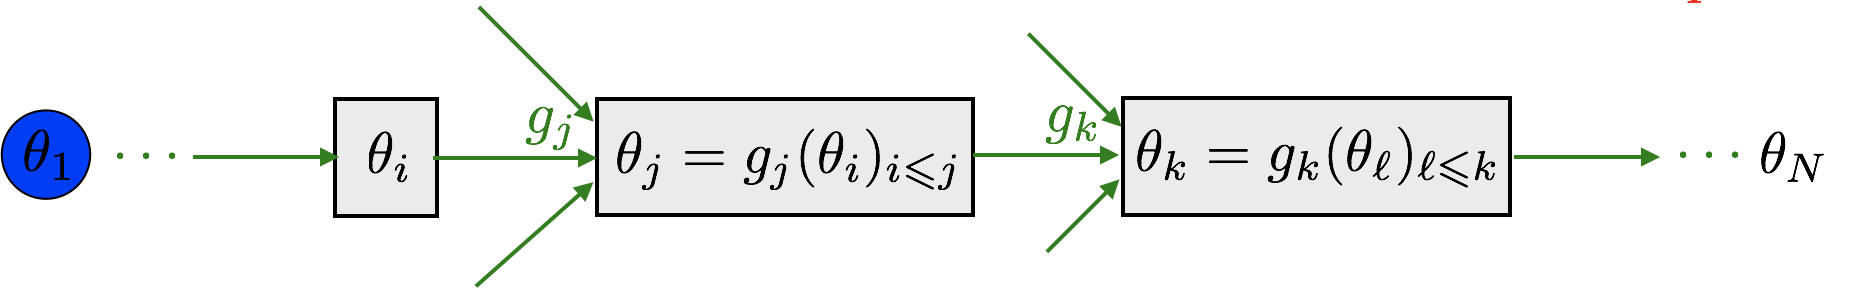
\includegraphics[width=.7\linewidth]{auto-diff/dag-element}}
\hbox{}\vspace{3mm}\hbox{}
\fbox{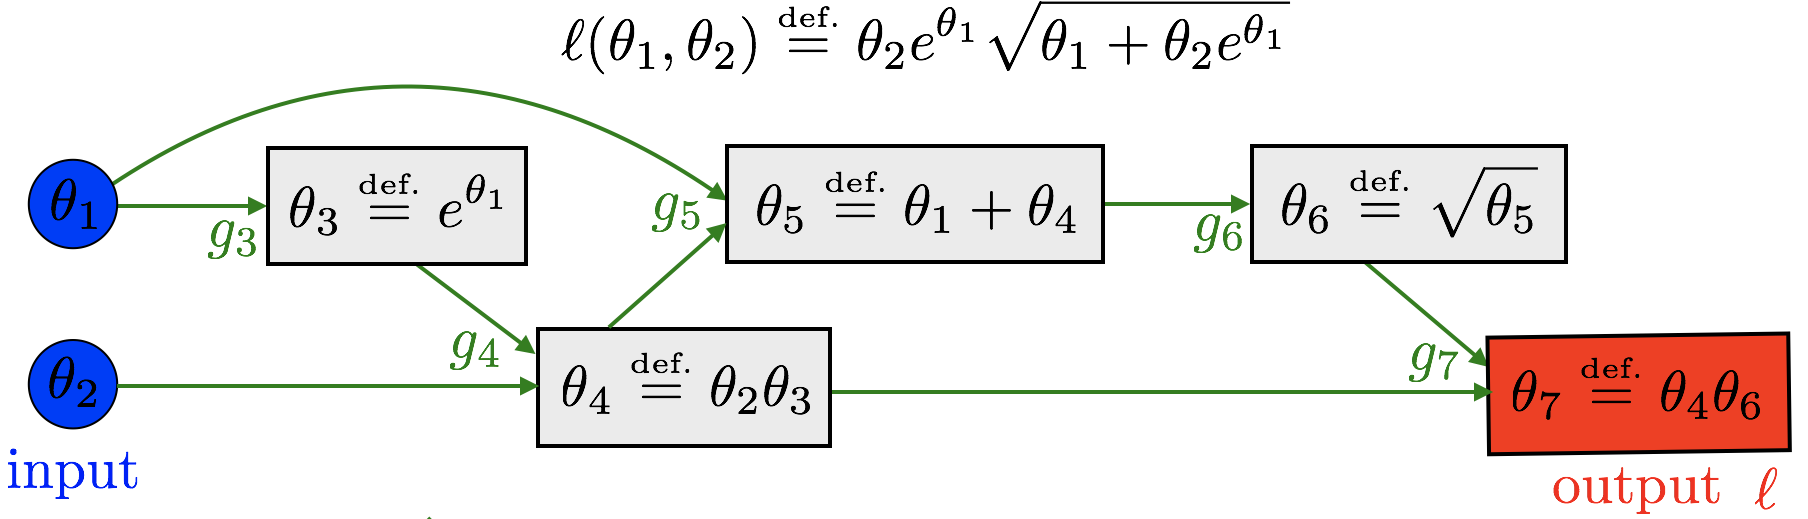
\includegraphics[width=.7\linewidth]{auto-diff/dag-example}}
\caption{\label{fig-dag-example}
Top: elementary component of the DAG computational graph. 
Bottom: example of DAG computational graph.
}
\end{figure}

One can generalize the idea above to differentiate automatically any function which can be implemented on a computer. What is even more surprising is that the computational cost is the same as the one of evaluating the function itself. This fundamental computational fact (that gradient evaluation and function evaluation have the same computational cost) is not so well known, but is of paramount practical interest when it comes to differentiating complicated recursive functions. We will apply it in a very simple setup for deep-architectures, but it can be applied to much more involved computational architectures. 

Note that this results only applies for function which output scalar values. For functions which output vector values, one can of course re-use this idea for each output, but this is in general vastly sub-optimal, because it ignore the redundancy between the computation of each output. The determination of optimal strategy in this case is known to be NP-hard. This include for instance the computation of the Hessian of a scalar valued function (since it corresponds to the differentiation of the gradient, which is itself a vector-valued function). Fortunately, for machine learning application, one is often interested in differentiating only empirical losses functions, which as scalar valued.

%%%%
\paragraph{Forward pass as a DAG traversal.}

The crux of this idea is that the computational flow of any computable function $\ell$ can be represented as a directed acyclic graph. 
%
We denote $(\th_i)_{i=1}^R$ the set of all scalar variables (input, output and intermediary) manipulated by the computational program.
%
Without loss of generality, we impose that the first variable $(\th_1,\ldots,\th_M)$ are the $M$ input variables, while the last $\th_R$ is the output variable. The function to be computed is thus of the form 
\eq{
	\th_R = \ell( \th_1,\ldots,\th_M )
}
where $\ell : \RR^M \rightarrow \RR$ is broken in $R-M+1$ intermediate steps corresponding to all the remaining variable $(\th_i)_{M < i < R}$. 
%
The successive execution of the program defines an ordering of all the intermediate variables, so that, after initializing the input variables $(\th_1,\ldots,\th_M)$, the forward pass computes the value of $\th_r$ for $r=M+1,\ldots,R$ as
\eq{
	\th_r = g_r( \th_{\pi(r)} )
}
for some scalar valued function $g_r : \RR^{|\pi(r)|} \rightarrow \RR$, where $\pi(r) \subset \{1,\ldots,r-1\}$ is the set of ``parent'' node of $r$ in a directed acyclic graph (DAG).  Figure~\ref{fig-dag-example} shows an example of such a computational DAG.


From a symbolic computation point of view, variables $\th_j$ (for $j>M$) in the graph can be interpreted either as variables (i.e. which can be assigned scalar values) and functions depending on input variables $\th_m$ for $m \leq M$. 
% 
The beauty of this DAG representation is that one can also view $\th_j$ as depending on any other intermediate variable $\th_i$ as long as $i<j$. 

%%%%
\paragraph{Direct mode auto-diff.}

The goal is to compute the gradient vector, which reads
\eq{
	\nabla \ell =  \pa{ \pd{\th_R}{\th_m} }_{m=1}^M. 
}
The naive way to comput this gradient vector would thus be to compute for each of the $M$ input variable $\th_m$ the differential $\pd{\th_j}{\th_m}$ of all function $\th_j$ with respect to $\th_m$. Without loss of generality, we consider $m=1$. This can be achieved by using the standard chain rule
\eql{\label{eq-chain-rule-forward}
	\pd{\th_j}{\th_1} = \sum_{i \in \pi(j)} \pd{\th_j}{\th_i} \pd{\th_i}{\th_1}.
}
Here the multipliers involved are actually differential of the elementary functions
\eq{
	\pd{\th_j}{\th_i} = \partial_i g_j
} 
Note that this writing is abusive, since $\pd{\th_j}{\th_i}$ really means that in practice such a differential is evaluated assuming all the variable $(\th_r)_{r<j}$ on which the function  $\th_j$ depends are defined to their respective value (which have been computed by the forward pass, which here can be run in parallel to the forward DAG traversal).

By traversing forward the DAG, iterating this formula compute all the derivative, and in particular $(\nabla \ell)_1 = \pd{\th_R}{\th_1}$. 
%
This approach, while being the most natural, is however vastly sub-optimal because its complexity is $M$ times the one of the evaluation of the function. 

%%%%
\paragraph{Reverse mode auto-diff.}

Instead of computing the quantities $(\pd{\th_j}{\th_1})_j$, a radically different approach consists in rather computing the quantities $\pd{\th_L}{\th_j} = (\nabla \ell)_j$. In place of the ``forward'' chain rule, one needs to the backward one
\eql{\label{eq-chain-rule-forward}
	\pd{\th_R}{\th_j} = \sum_{j \in \pi(k)} \pd{\th_R}{\th_k} \pd{\th_k}{\th_j}.
}
Note that here the summation is done over $k$ which are ``child'' of $j$ in the DAG. Here the multiplier appearing in the formula are differential of the elementary function since $\pd{\th_k}{\th_j} = \partial_j g_k$. 
%
The main interest of this reverse recursion~\eqref{eq-chain-rule-forward} with respect to the direct one~\eqref{eq-chain-rule-forward} is that it only needs to be run once, so that the overall complexity is the same as the one of the forward pass to compute the function itself. 

Figure~\ref{fig-fwdbwd} recaps the two passes of the reverse mode automatic differentiation method.

\begin{figure}
\centering
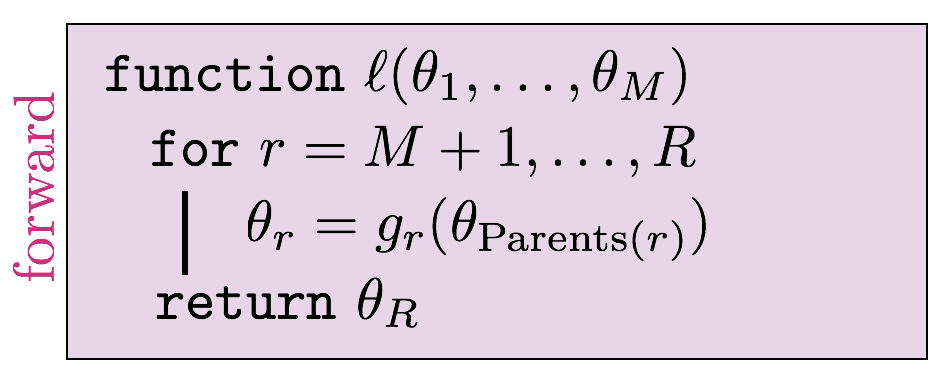
\includegraphics[width=.4\linewidth]{auto-diff/forward}
\qquad
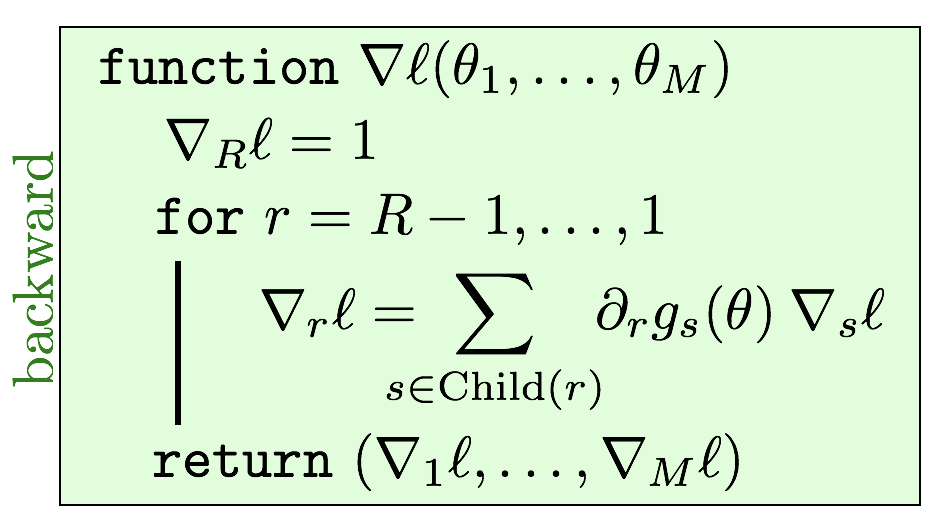
\includegraphics[width=.4\linewidth]{auto-diff/backward}
\caption{\label{fig-fwdbwd}
Recap of the two step of the automatic differentiation procedure.
}
\end{figure}

The main bottleneck of this backward automatic differentiation technic is the memory consumption. Indeed, since all intermediate results need to be computed and stored explicitly before applying the backward pass, memory grows proportionally to execution time. This can be unacceptable for very large machine learning model. Fortunately, it is possible to trade time vs. memory and only keep track of a fraction of intermediate results, and retrieve the missing result locally by small forward passes. Doing this approach recursively allows to only have a logarithmic overhead in term of both time and memory, showing the vast superiority of automatic differentiation method with respect to any other alternative for differentiation. We could not insist more on the crucial importance and impact of this class of technics on modern data science. 